\documentclass{beamer}
\usepackage[utf8]{inputenc} 
\usepackage[T1]{fontenc}
\usepackage{lmodern}
\usepackage{import}

\subimport{.}{header}

\usepackage{graphicx}
\usepackage{geometry}

\usepackage[sort]{natbib}
\bibliographystyle{plain} % Or your specific bibliographystyle
%\setcitestyle{authoryear,open={((},close={))}}

\def\newblock{} % To avoid a compilation error about a function \newblock undefined

\usepackage{setspace}


\makeatletter
\setbeamertemplate{footline}
{
    \leavevmode%
    \hbox{%
        \begin{beamercolorbox}[wd=.333333\paperwidth,ht=2.25ex,dp=1ex,center]{author in head/foot}%
            \usebeamerfont{author in head/foot}\insertshortauthor
        \end{beamercolorbox}%
        \begin{beamercolorbox}[wd=.333333\paperwidth,ht=2.25ex,dp=1ex,center]{title in head/foot}%
            \usebeamerfont{title in head/foot}\insertshorttitle
        \end{beamercolorbox}%
        \begin{beamercolorbox}[wd=.333333\paperwidth,ht=2.25ex,dp=1ex,right]{date in head/foot}%
            \usebeamerfont{date in head/foot}\insertshortdate{}\hspace*{2em}
            \insertframenumber{} / \inserttotalframenumber\hspace*{2ex} 
        \end{beamercolorbox}}%
        \vskip0pt%
    }
    \makeatother

\setlength{\abovecaptionskip}{0pt}

\hypersetup{%
  colorlinks=true,
  linkcolor=blue,
  urlcolor=blue,
  urlbordercolor=red% hyperlink borders will be red
}
\usepackage{bbding}

\title{Weak nuclear interactions in Core-Collapse supernovae}
\subtitle{Accouting for the full nuclei distribution}
%\author[Lucas Gautheron, Lydia Roos, Martin White, Yee Yap]{Lucas Gautheron\inst{1} \and Bogdan Malaescu\inst{1} \and Lydia Roos\inst{1} \and Martin White\inst{2} \and Yee Yap\inst{1}}
%\institute[]{\inst{1}LPNHE \and \inst{2}University of Adelaide}
\date{}

\AtBeginSection[]
{
  \begin{frame}<beamer>{Outline}
    \tableofcontents[currentsection,currentsubsection]
  \end{frame}
}

\begin{document}

\begin{frame}
\titlepage
\end{frame}

\begin{frame}
\frametitle{Outline}
\tableofcontents
\end{frame}

\section{Problem space}
\subsection{Interactions and hypotheses}


\begin{frame}
\frametitle{Interactions and model}

Interactions studied:
\begin{itemize}
\item \textbf{Neutrino-nucleus elastic scattering}: $\nu + X \to \nu + X$ ($\nu = \nu_e, \bar{\nu_e}, \nu'$)
\item \textbf{Electron-capture}: $^{A}_{Z} X + e^{-} \to ^{A}_{Z-1} X' + \nu_e$
\end{itemize}

Hypotheses:
\begin{itemize}
\item All reactions in thermodynamic equilibrium except for weak interactions
\item The neutrino gas follows a fermi-dirac distribution with effective potential $\mu^{eff}_e$ (``Leakage scheme'')
\item Assumes nuclei distribution is equivalent to average nucleus $a_{heavy} = \langle A \rangle$, $z_{heavy} = \langle Z \rangle$. (=SNA, Single Nucleus Approximation)
\end{itemize}
\end{frame}

\begin{frame}
\frametitle{Interactions and model}

Interactions studied:
\begin{itemize}
\item \textbf{Neutrino-nucleus elastic scattering}: $\nu + X \to \nu + X$ ($\nu = \nu_e, \bar{\nu_e}, \nu'$)
\item \textbf{Electron-capture}: $^{A}_{Z} X + e^{-} \to ^{A}_{Z-1} X' + \nu_e$
\end{itemize}

Hypotheses:
\begin{itemize}
\item All reactions in thermodynamic equilibrium except for weak interactions
\item The neutrino gas follows a fermi-dirac distribution with effective potential $\mu^{eff}_e$ (``Leakage scheme'')
\item \sout{Assumes nuclei distribution is equivalent to average nucleus $a_{heavy} = \langle A \rangle$, $z_{heavy} = \langle Z \rangle$. (=SNA, Single Nucleus Approximation)}
\end{itemize}
\end{frame}

\begin{frame}
\frametitle{Questions}
\begin{itemize}
\item How important is the impact on interactions strength?
\item How important is the impact on supernova simulations ? $(Y_e, L_\nu)$...
\end{itemize}
\end{frame}

\subsection{Program structure}

\begin{frame}
\frametitle{Program structure}

\begin{itemize}
\item An external program computes electron-capture rates and scattering cross-sections for each $(T, n_b, Y_e, \mu_{nu}^{eff})$ of the phase-space.
\begin{itemize}
\item Input: CompOSE tables (including nuclei distribution)
\item Output: HDF5 format tables containing capture rates $\lambda_{ec}$ and scattering cross-sections $\sigma$
\end{itemize}
\item CoCoNuT imports these tables and use quadrilinear interpolation to recover $\sigma$'s and $\lambda_{ec}$ (\small neutrino scattering on the nucleus -  cross-sections used to be calculated on the fly \normalsize )
\end{itemize}
\end{frame}

\section{Neutrino scattering}

\subsection{Expression}

\begin{frame}
\frametitle{Cross-section expression}

Same as employed in \cite{these_peres}.

\begin{align}
\sigma(A,Z)& = \dfrac{\sigma_0  A^2  \epsilon_\nu^2}{m_e} Y_{X}n_b \dfrac{F_5(\mu_\nu/T)}{F_3(\mu_\nu/T)} \\
& \times \left [ (C_A-C_V)+(2-C_A-C_V)\dfrac{2Z-A}{A} \right ]^2\\
& \times  \dfrac{ f( r_X^2 \epsilon_\nu^2 )}{1+\exp(-\epsilon_\nu/T)}
\end{align}

$\Longrightarrow$ SNA $\to$ $\sum_{A,Z}$

\end{frame}

\subsection{Results}

\begin{frame}
\frametitle{$\sigma_{scattering}$}
0.01 MeV $< T <$ 5 MeV,  $10^{-8} \textrm{fm}^{-3} < n_b < 10^{-2} \textrm{fm}^{-3}$, $Y_e > 0.1$
\vspace{-3em}
%\begin{figure}
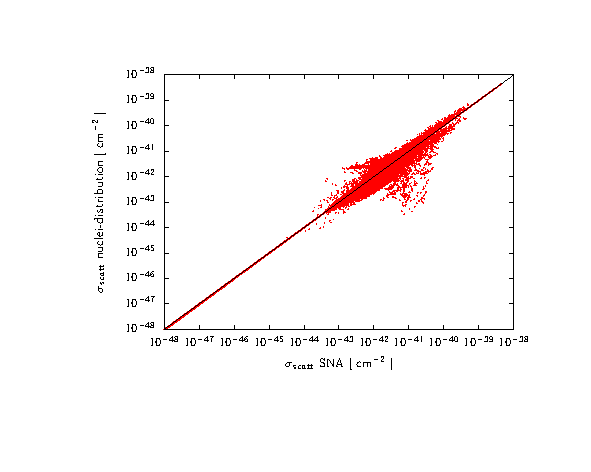
\includegraphics[width=1.1\textwidth]{plots/scattering_xs.pdf}
%\end{figure}
\end{frame}

\begin{frame}
\frametitle{Impact on supernova}
$M = \textrm{40} M_{\odot}$
\vspace{-3em}
%\begin{figure}
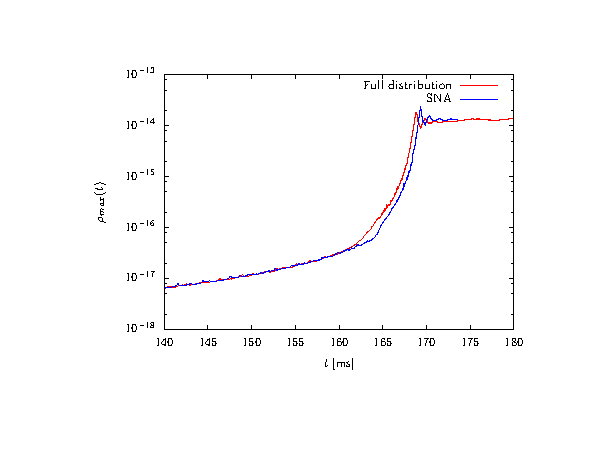
\includegraphics[width=1.1\textwidth]{plots/rho.pdf}
%\end{figure}
\end{frame}

\begin{frame}
\frametitle{Impact on supernova}
$M = \textrm{40} M_{\odot}$
\vspace{-3em}
%\begin{figure}
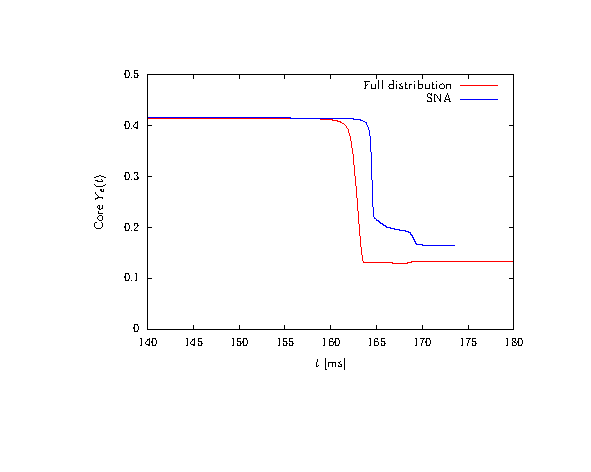
\includegraphics[width=1.1\textwidth]{plots/y_e.pdf}
%\end{figure}
\end{frame}

\section{Electron capture}

\subsection{Expression}

\begin{frame}
\frametitle{Rate expression}

Previously used Bruenn 1985\cite{bruenn}

\begin{itemize}
\item proton capture ($p+e^{-}\to n+\nu_e$): unchanged
\item nucleus capture: B. Peres used Bruenn expr. with shell blocking effect: 
\begin{align*}
\lambda(A,Z) & = \dfrac{7G_F^2}{\pi^2}Y_X |V_{ud}|^2 g_A^2\\
& \times \mathcal{N}(Z,N)\\
& \times \dint E^2(E+Q)^2 \sqrt{1-\dfrac{m_e^2}{(E+Q)^2}} \\
& \times \ \ S(E+Q,\mu_e) (1-S(E,\mu_{\nu})) \dd E
\end{align*}
\end{itemize}

$\Longrightarrow$ Shell effect shown to be removed at high densities
\newline
$\Longrightarrow$ SNA $\to$ $\sum_{A,Z}$

\end{frame}

\begin{frame}
\frametitle{Rate expression}

$\Longrightarrow$ full expression too expensive to compute.
\newline
Instead: Parametrization by Langake et al.

\begin{equation}
\lambda = \dfrac{\beta \ln 2}{K} \left (\dfrac{T}{m_e}\right)^5 \left (F_4(\eta)-2\chi F_3(\eta)+\chi^2 F_2(\eta)\right)
\end{equation}

($\chi = (Q-\Delta E)/T$, $\eta = \chi +\mu_e/T$, $F_i(t) = \dint_{0}^{+\infty} \dfrac{x^i dx}{1+\exp(x-t)}$).

$\Longrightarrow$ Problem: doesn't account for $\nu$ blocking. Suggested param alternative:

\begin{equation}
\lambda = \dfrac{\beta \ln 2}{K} \left (\dfrac{T}{m_e}\right)^5 \dint_{0}^\infty 
\end{equation}
\end{frame}

\section{Next}

\begin{frame}
\frametitle{Next}
\begin{itemize}
\item Electron capture: test parametrization relevance
\item Electron capture: impact on collapse simulations
\item Compute $L_\nu$
\end{itemize}
\end{frame}


\begin{frame}[allowframebreaks]
        \frametitle{References}
        \bibliography{presentation}
\end{frame}



\section{Appendices}

\begin{frame}
\frametitle{$a_{heavy}$/$z_{heavy}$ problem}
0.01 MeV $< T <$ 5 MeV,  $10^{-8} \textrm{fm}^{-3} < n_b < 10^{-2} \textrm{fm}^{-3}$, $Y_e > 0.1$
\vspace{-3em}
%\begin{figure}
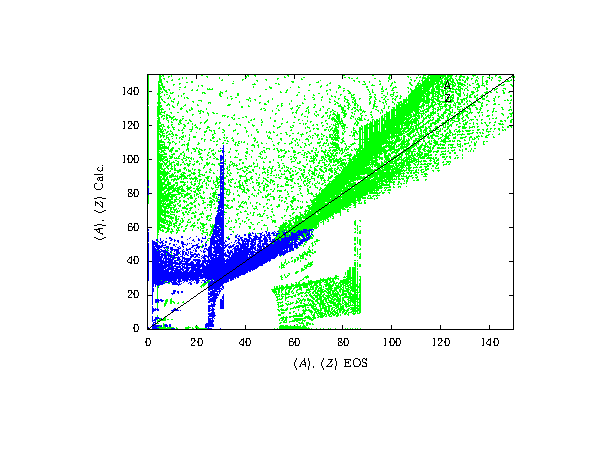
\includegraphics[width=1.1\textwidth]{plots/abundances.pdf}
%\end{figure}
\end{frame}

%\begin{frame}
%\frametitle{Bugfix for $q\bar{q}\to G*$ cross-section in Pythia 8.212}
%
%\begin{columns}
%\begin{column}{0.6\linewidth}
%\begin{itemize}
%\item Pythia \textbf{8.212} changelog comes with :
%{\tiny Minor correction in the cross section for ffbar -> G* for extra-dimensional processes.\normalsize}
%\item The code difference is :
%\tiny
%\texttt{diff pythia8210/src/SigmaExtraDim.cc pythia8212/src/SigmaExtraDim.cc}
%
%\texttt{290c290}
%
%\texttt{ <   sigma0          = widthIn * sigBW * widthOut * sH / m2Res;}
%
%\texttt{\ \ \  sigma0          = widthIn * sigBW * widthOut;}
%\normalsize
%$\Rightarrow$ Removal of redundant $m_{\gamma\gamma}^2/m_{G}^2$ factor.
%\item Confirmed as a bugfix by Stephen Mrenna from Pythia team.
%\item Official EVNT samples from central production used \textbf{8.186}
%\item Pythia \textbf{8.212} available in AtlasProduction \textbf{19.2.5.9} (built last week)
%\end{itemize}
%\end{column}
%\begin{column}{0.45\textwidth}
%Pythia 8.210, \textcolor{red}{Red} = Correct distribution. \textcolor{green}{Green} = $m_{\gamma\gamma}^2/m_{G}^2 \times $ \textcolor{red}{Red}.
%    \centering
%     \includegraphics[width=0.9\linewidth]{plots/PythiaS_304869_qq_mgg9.png}
%
%    \centering
%
%     \includegraphics[width=0.9\linewidth]{plots/PythiaS_304869_gg_8210.png}
%\end{column}
%\end{columns}
%\end{frame}
%
%
%\begin{frame}
%\frametitle{Backups - parton lumi parametrization fidelity}
%\begin{figure}
%    \centering
%     \includegraphics[width=0.8\linewidth]{plots/lum_param.pdf}
%    \caption{PDF luminosity functions from APFEL using the same PDF set as Pythia, compared to our quick parametrization, for $gg$ and $q\bar{q}$. ($\mathcal{L}_{\mbox{param}}/\mathcal{L}_{\mbox{APFEL}}$)}
%\end{figure}
%\end{frame}


\end{document}


